\documentclass[12pt]{article}
\usepackage{amsmath}
\usepackage{amsfonts}
\usepackage{amssymb}
\usepackage{graphicx} 

\title{Properties of numerical integrators}
\author{Les Schaffer\\ Joseph Shearer}


\begin{document}
\maketitle
\section{Numerical integration of a single first order ODE}
Let's take the differential equation
\begin{align}
\frac{dy}{dx}&=-y\\
y(x=0)&=y_0
\end{align}
It has a solution $y(x) = y_0\, e^{-x}$; what if we try to approximate the solution numerically? 

The standard approach is to approximate the derivative as $dy/dx\approx (y_{n+1} - y_n)/\Delta x$ so that the differential equation is converted to a finite difference equation $(y_{n+1} - y_n)/\Delta x = - y_n$ to produce the algorithm:
\begin{align}
y_{n+1} &= y_n - \Delta x\, y_n\\
y_0 &= y_0
\end{align}
We can solve the recurrence relation (3) exactly:
\begin{equation}
y_{n+1} = (1-\Delta x) y_n \Longrightarrow y_n = (1-\Delta x)^n y_0
\end{equation}
There are five cases: $0<\Delta x<1$, $\Delta x = 1$, $1<\Delta x <2$, $\Delta x = 2$, and $\Delta x > 2$. Their properties, letting $0<\alpha<1$ and $\beta>1$:
\begin{align}
y_n &= \alpha^n\, y_0 \quad\hbox{\rm decreases monotonically to zero}\\
y_n &= 0 \quad \hbox{\rm for $n>=1$}\\
y_n &= (-\alpha)^n\, y_0 \quad\hbox{\rm decreases by oscillation around zero, to zero}\\
y_n &= (-1)^n\, y_0\quad\hbox{\rm for all $n>=1$}\\
y_n &= \beta^n\, y_0\quad\hbox{\rm increases monotonically to  $\pm\infty$}
\end{align}
Only the case $\Delta x < 1$ corresponds with the real solution.

\section{Improvements to first order numerical solutions}
Is there a way to improve the performance of the first order solution? Consider the implicit method
\begin{align}
\frac{dy}{dx} \approx (y_{n+1}-y_n)/\Delta x &= - y_{n+1}\\
(1+\Delta x)\, y_{n+1} &= y_n\\
y_n &= \left(\frac{1}{1+\Delta x}\right)^n\, y_0
\end{align}
which decreases to zero for all values of $\Delta x$!!! This method does not have any of the oscillatory or instability behavior of the first method. 

A comparison of the exact, numerical (eq. 5) and implicit numerical (eq. 13) is shown in Figure 1, for $y_0=1$ and $\Delta x=1.8$,  which puts us in the behavior described in eq. 8 for the first numerical scheme. Notice how the implicit scheme still does a decent job of describing the exponential decrease. 
\begin{figure}[ht]
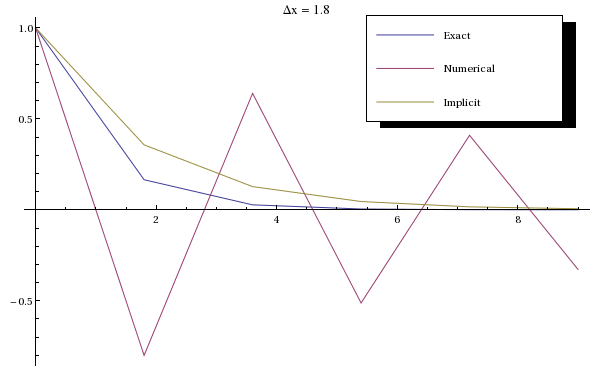
\includegraphics[scale=0.65]{ode1.png} 
\caption{Comparison of standard and implicit numerical scheme for $\Delta x=1.8$, along with exact solution to differential equation. for $y_0=1$.  }
\end{figure}
Similarly, Figure 2 compares the behavior of the first numerical scheme (eq. 5) with the implicit scheme, where the $\Delta x$ of the latter is $4$ times that of the former. Clearly the implicit solution does a better job for larger $\Delta x$. 
\begin{figure}[ht]
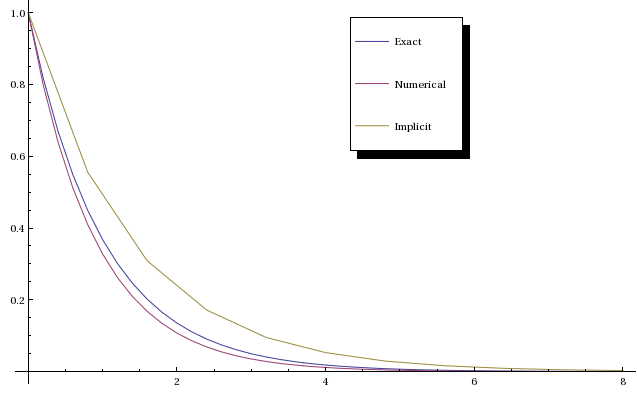
\includegraphics[scale=0.65]{ode2.png} 
\caption{Comparison of implicit ($\Delta x=0.8$) to standard $(\Delta x=0.2)$ numerical scheme for $y_0=1$, along with exact solution to differential equation. }
\end{figure}

\section{Error analysis}
 We can compare the numerical solution to the exact solution, at the points $x$ calculated numerically:
\begin{equation}
y_n/(y_0\, e^{-x})_{x=x_n} = (1-\Delta x)^n e^{n\Delta x}
\end{equation}
which goes to $1$ {\it only} as $\Delta x\to 0$. 

Note that for $dy/dx = y$, 
\begin{equation}
y_n = (1+\Delta x)^n y_0
\end{equation}
which does grow like the exact solution $y_0 \, e^x$. The fractional error is
\begin{equation}
(y_0\, e^x - y_n)/(y_0\, e^x) = 1 - (1+\Delta x)^n e^{-n \Delta x}
\end{equation}
To be continued ... 
\end{document}